\graphicspath{{./Sections/Chapter1_intro/figures/}}
\chapter{Introduction}
\section{A primer on superhydrophobic surfaces}\label{S:Ch1:superhydrophobic}
This thesis is concerned with droplet transport in response to flexible boundaries. However, the motivation for studying this comes from manufacturing superhydrophobic surfaces that are not compromised by the condensation of vapour. This section provides a brief background to the rapidly expanding field of superhydrophobic surfaces. A more detailed overview can be found in the review paper by~\cite{Simpson2015RepProgPhys}, for example.

\begin{figure}[t]
\centering
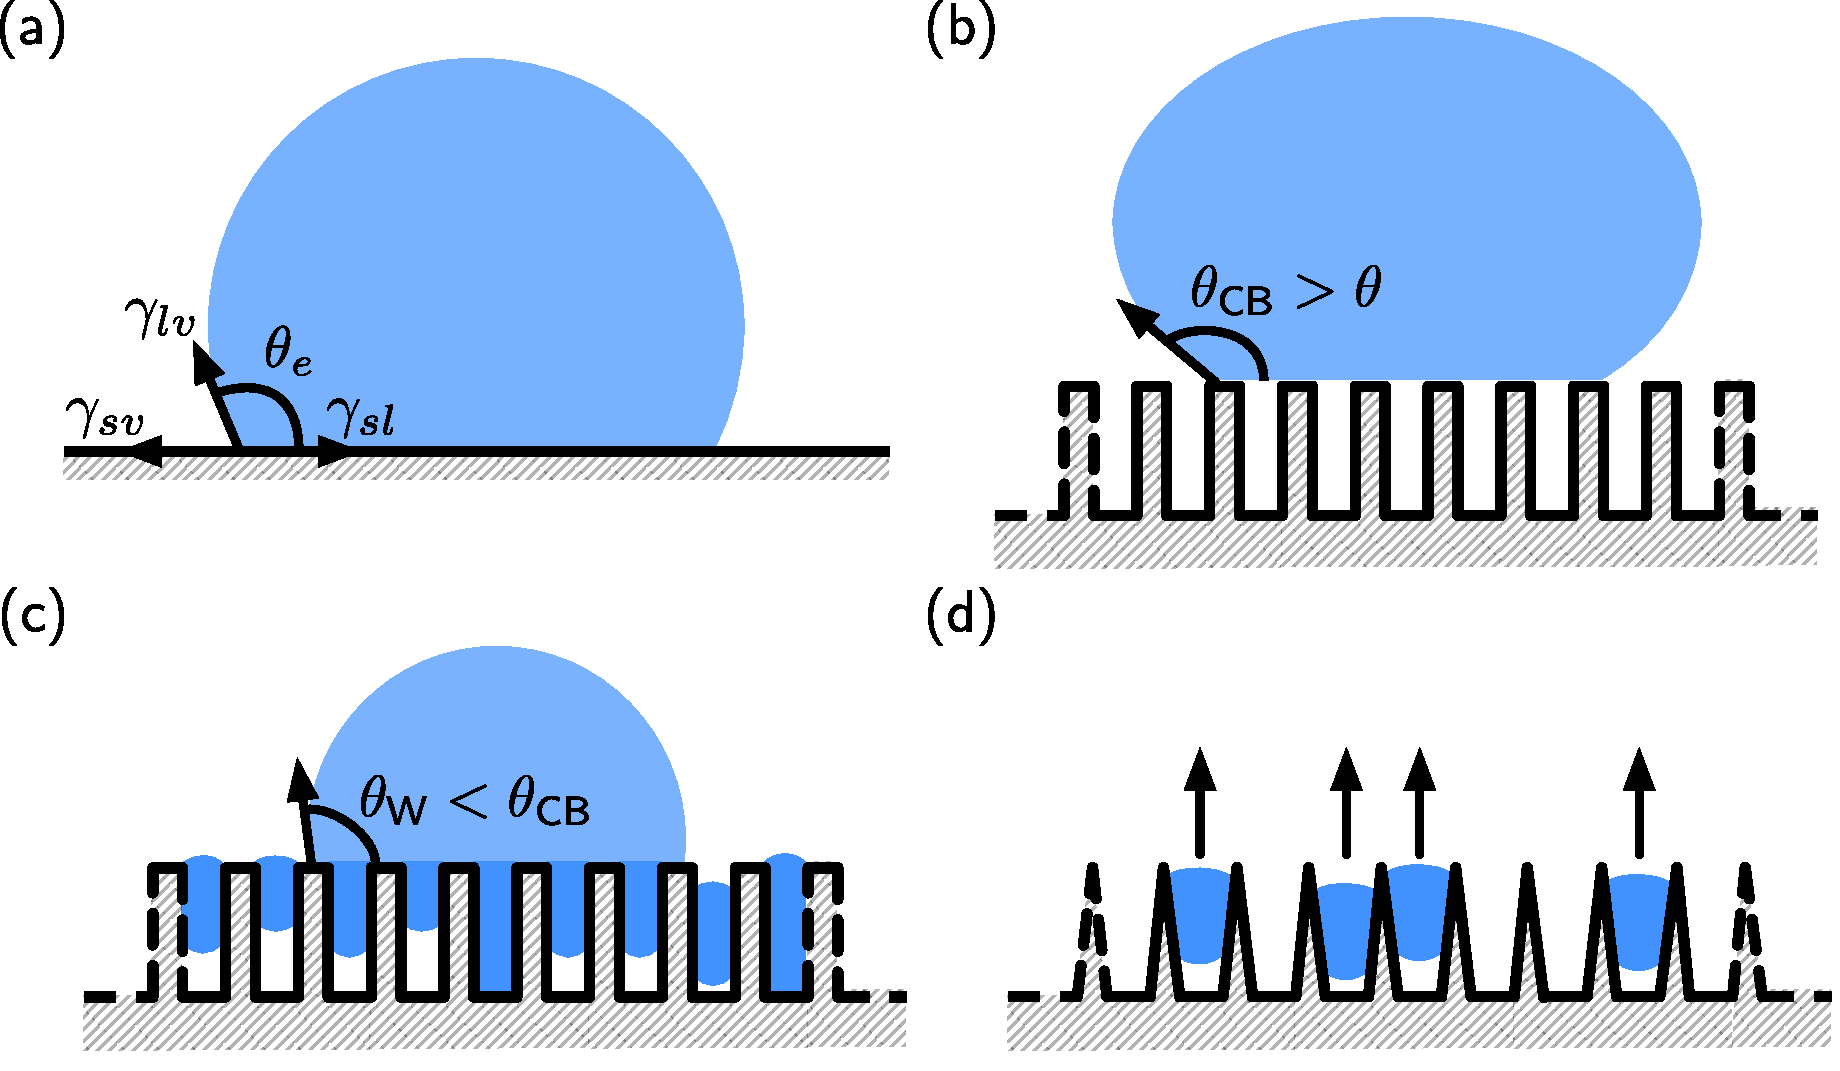
\includegraphics[scale=0.42]{Texturing}
\caption{(a) A sessile droplet on a solid surface takes the macroscopic contact angle $\theta_e$ that results in a balance between the  liquid-vapour, solid-liquid, and solid-vapour interfacial energies $\gamma_{lv}$, $\gamma_{sl}$, and $\gamma_{sv}$, respectively, according to Young's equation~\eqref{E:Ch1:Young}. (b) A droplet perched on top of topographical structures in a Cassie-Baxter state makes a macroscopic contact angle greater than that specified by Young's equation. (c) If the droplet (light blue) contacts a surface whose topographical features contain condensed droplets (dark blue), it is in a Wenzel state, characterized by a lower macroscopic contact angle (compared to a Cassie-Baxter state) and reduced mobility. (d) If the topographical features are conically shaped, fewer droplets condensate between them, and those that do may be driven out of the channels that exist between features.}\label{fig:Ch1:Textured}
\end{figure}



Informally, superhydrophobic surfaces are characterized by the observation that water droplets placed on them take almost ball-like shapes, and roll or slide off easily. As they do so, droplets may entrain surface contaminants, effectively cleaning the surface~\citep{Blossey2003Nature}. For this reason, superhydrophobic surfaces can be considered a class of `self-cleaning' surfaces~\citep{Liu2012AnnRevMaterSci}. A  familiar natural example of a superhydrophobic self-cleaning surface is the leaf of the lotus plant (\textit{Nelumbo nucifera})~\citep{Barthlott1997Planta}; indeed, self cleaning surfaces are often said to exhibit `the lotus effect'~\citep{Marmur2004Langmuir}. Nevertheless, superhydrophobic surfaces have a wide range of applications beyond self-cleaning, including corrosion resistance~\citep{Liu2011Nanoscale}, drag reduction~\citep{McHale2010SoftMatter}, and anti-icing~\citep{Meuler2010ACSnano}.

%but they're more useful than just as self-cleaning  surfaces --.> artificial examples

%A surface is rendered superhydrophobic using a combination of surface texturing and chemistry
% \red{what happens on a flat surface, and flat cannot be superhydrophobic}
\subsubsection{Contact angles on superhydrophobic surfaces}
The heuristic notion of superhydrophobicity introduced above is made more formal by introducing the contact angle $\theta$: the macroscopic angle that a sessile droplet makes with a surface; a surface is superhydrophobic if it has a contact angle $\theta > 150\si{\degree}$~\citep{Ma2006CurrOpCollSci}.

If the surface is homogeneous and smooth, and the droplet is in equilibrium, the contact angle is the Young angle $\theta_e$, which is set by the material properties via Young's equation~\citep{Young1805PhilosTrans, deGennes1985RevModPhy},
 \begin{equation}\label{E:Ch1:Young}
 \cos \theta_e = \frac{\gamma_{sv} - \gamma_{sl}}{\gamma_{lv}}.
 \end{equation}
Here $\gamma_{sv}, \gamma_{sl}$, and $\gamma_{lv}$ are the interfacial energies at the solid-vapour, solid-liquid, and liquid-vapour interfaces (Figure~\ref{fig:Ch1:Textured}(a)).

In reality, however, surfaces are heterogenous, and droplets are not always in equilibrium. In these cases, the contact angle is not unique: if the droplet's contact line (the line of contact between solid and liquid) is stationary, it's contact angle can take any value between an advancing angle, $\theta_a$, and a receding angle, $\theta_r$. In addition, if the contact line is advancing, the contact angle takes this advancing angle and if the contact line is receding, the contact angle takes the receding angle. The contact angle hysteresis is defined as the difference between these angles, $\theta_a - \theta_r$. Superhydrophobic surfaces typically exhibit low contact angle hysteresis (superhydrophobic surfaces with a contact angle hysteresis less than $\si{10\degree}$ are said to be super-repellent~\citep{Attinger2016Nanoscale}).

\subsubsection{Making superhydrophobic surfaces}
The maximum Young angle that has been achieved using known materials and a water droplet is approximately $ 120\si{\degree}$~\citep{Blow2010Langmuir}. Nevertheless, many examples of surfaces with contact angles approaching 180$\si{\degree}$ exist. Such large contact angles can be achieved by introducing topographical features to the surface~\citep{Bico2001EPL}: droplets are able to perch on top of features in a so called Cassie-Baxter state~\citep{Cassie1944TransFaraday,Cassie1948FaradayDiscuss}; their macroscopic contact angle is increased, compared to a flat surface, because much of the solid-liquid contact has replaced by liquid-air contact (Figure~\ref{fig:Ch1:Textured}(b)). Explicitly, the contact angle of a droplet in a Cassie-Baxter state, $\theta_{\text{CB}}$, satisfies~\citep{Lafuma2003NatureMat}
\begin{equation}
\cos  \theta_{\text{CB}} = \phi \cos \theta_e - (1-\phi)
\end{equation}
where $\phi$ is the fraction of the footprint of the droplet in contact with the solid surface. The lotus leaf, for example, employs a hierarchical structure of papillose epidermal cells~\citep{Neinhuis1997AnnBot} to increase
surface roughness, resulting in contact angles above 160$\si{\degree}$~\citep{Barthlott1997Planta}. By modifying the surface topography, surfaces demonstrating contact angles all the way up to 180\si{\degree}, the maximum possible, have been manufactured~\citep{Bico1999EPL, Quere2005RepProgPhys}.

\subsubsection{Textured superhydrophobic surfaces fog up}
One major limitation of using texturing to create superhydrophobic surfaces is their tendency to ‘get wet’ when exposed to foggy or humid environments -- droplets of a size comparable to the scale of the texturing nucleate and grow within it, destroying the Cassie-Baxter state~\citep{Dorrer2007Langmuir,Varanasi2009APL}. Macroscopic droplets subsequently deposited on the surface come into contact with existing liquid bridges embedded within the texturing (Figure~\ref{fig:Ch1:Textured}(c)), thereby becoming a `Wenzel' state~\citep{Wenzel1949JPhysChem}. The contact angle $\theta_{\text{W}}$ of a droplet in a Wenzel state satisfies
\begin{equation}
\cos \theta_{\text{W}} = r\cos \theta_e,
\end{equation}
where $r>1$ is the ratio of the actual surface area to apparent surface area of the texturing. A droplet in a Wenzel state has significantly reduced mobility, compared to a Cassie-Baxter state -- the contact angle is lower, and the droplet may pin strongly on the topographical features, leading to a significantly increased contact angle hysteresis. Lotus leaves, for example, have been observed to experience an increase in their roll off angle (the angle that the surface must be rotated to in order to initiate rolling, a measure of contact angle hysteresis) from $\lesssim$~\si{5~\si{\degree}} to above 70\si{\degree} when droplets are condensed, rather than deposited, onto their surface~\citep{Cheng2005aAPL,Cheng2005bAPL}.

Of course, nature experiences this same problem and has found at least one solution: by tailoring the shape of the topographical structures, fog build-up can be reduced. For example, the texturing on  the superhydrophobic wings of some cicada~\citep{Wisdom2013PNAS} and butterflies~\citep{Chen2018PLOSone} features conical structures (shown schematically in Figure~\ref{fig:Ch1:Textured}(d)). These structures are believed to reduce the total  number of nucleating droplets because there is less room for condensation to occur near the base of the cones~\citep{Xu2016RSCadv}.  In addition, droplets that bridge between two neighbouring cones may be spontaneously propelled towards their tips (i.e.~away from the surface). Droplets can be removed from the tips by mechanical actuation or by spontaneous jumping after coalescing with an adjacent droplet~\citep{Boreyko2009PRL, Boreyko2010PhysFlu} (coalescing with another droplet releases surface energy, which is converted into kinetic energy). By mimicking these natural structures,  artificial superhydrophobic surfaces with conically shaped protrusions have been shown to perform significantly better in foggy conditions than superhydrophobic surfaces with cylindrical features~\citep{Mouterde2017NatMater}.

The above example of antifogging of a superhydrophobic surface is facilitated by spontaneous droplet transport in response to the geometric gradient that arises when a droplet bridges two neighbouring cones. Such motion driven by geometric gradients is  one of a number of mechanisms for transporting droplets. We discuss these mechanisms in more detail next.

\section{Droplet transport}
%Moving small droplets: dominated by surface tension.
Liquid droplets experience body forces (gravity) and surface forces (surface tension). If a droplet has a typical length scale $L$, then body forces scale with $L^3$, while surface forces scale with $L^2$~\citep{deGennes2004}; this means that surface forces dominate the behaviour of sufficiently small droplets. The length scale below which surface tension dominates over gravity is the capillary length, $\ell_c = (\Delta \rho g/\gamma)^{1/2}$, where $\rho$ is the liquid density (assuming a negligible ambient density), $g$ is gravitation acceleration and $\gamma$ the interfacial tension coefficient~\citep{deGennes2004}. In this thesis, we are concerned with droplets of characteristic size below the capillary length.


%why do we care about moving small droplets
As we saw in \S\ref{S:Ch1:superhydrophobic}, control and transport of liquid droplets smaller than the capillary length is important in preventing fog build-up within the topographical features on superhydrophobic surfaces. More broadly, the transport of small droplets is critical in a wide range of applications including diagnostics~\citep{Yager2006Nature}, fog harvesting~\citep{Andrews2011Langmuir}, microfabrication~\citep{Srinivasarao2001Science}, and droplet-based microfluidics~\citep{Squires2005RevModPhys}.

%so if we want to move small droplets, we need to think about surface tension. we can either change the interfacial tension --> i.e. marangoni, or we can create a wettability gradient to create curvature differences on either side of the droplet and hence laplace pressure difference = flow. You can do this by making the contact angle vary across the droplet (e.g. chemical composition, nano-structuring gradients) or using geometry.

Liquid motion within a droplet is driven by gradients in the liquid pressure $p$. Locally, the droplet pressure (its Laplace pressure) is set by the surface tension $\gamma$ and interfacial curvature $\kappa$ according to the Young-Laplace equation $p = \gamma \kappa$~\citep{Laplace1799,Young1805PhilosTrans}. There are, therefore, two ways to generate droplet motion~\citep{Scriven1960Nature}: by creating gradients in surface tension, or by creating gradients in interfacial curvature.

Local variations in the surface tension, thereby generating a Marangoni flow within the droplet (towards regions of lower surface tension) exert a hydrodynamic force on the adjacent surface; the equal and opposite force applied by the surface propels the droplet along it.  Gradients in surface tension, or rather the associated Marangoni flow, can be created in droplets in a variety of ways including by varying the temperature across them (often called thermocapillarity)~\citep{Brzoska1993Langmuir, Pratap2008Langmuir}, by differential evaporation leading to differences in composition~\citep{Thomson1855}, by tailoring the surface chemistry~\citep{COTTINGTON1964, John2005EPJE}, and by using electrochemical effects~\citep{Gallardo1999Science}.


The second route to transporting small droplets is to create a gradient in the droplet's interfacial curvature. One way to do so is to vary the local contact angle; techniques such as electrowetting~\citep{Lippmann1875, Mugele2005JPhysCond}, variations in surface local topography~\citep{Shastry2006Langmuir}, surface chemistry~\citep{DosSantos1995PRL,Chaudhury1992Science,Daniel2001Science}, and surface photoirradiation~\citep{Ichimura2000Science} have all been successfully exploited to vary the local contact angle of, and thus transport, droplets.

Gradients in interfacial curvature can also be induced by the geometry of the adjacent surface. This method of droplet transport can be traced back three-centuries to Hauksbee~\citep{Hauksbee1710iii}, who observed that a droplet of oil between two non-parallel plates would  ``immediately move towards the touching side of the plane''. Droplet transport in similar tapered channels (wedges) has been studied in detail in more recent years by~\cite{Renvoise2009EPL} and~\cite{Reyssat2014JFM} and the mechanism is well understood: provided that the droplet wets (or has an affinity to) the walls of the channel, the negative interfacial curvature, whose magnitude is inversely proportional  to the local thickness of the wedge, is smaller (it is more negative) on the side of the droplet closest to the apex. The droplet is therefore `sucked' into the wedge. If, on the other hand, the droplet does not wet the channel walls, then the (positive) interfacial curvature is smaller at on the side furthest from the tip, where the channel is widest; non-wetting droplets are therefore squeezed out of the vertex. Crucially, we note that droplet motion in tapered channels is wettability-dependent -- wetting and non-wetting droplets move in opposite directions.

A similar mechanism is responsible for droplet propulsion from within a conically textured surface (Figure~\ref{fig:Ch1:Textured}(d)) -- the surface of the cones are themselves hydrophobic, so the droplets are pushed towards the weaker confinement at the top of the cones. Note, however, that if nucleating droplets consisting of a \textit{wetting} liquid were to bridge between two cones, the droplets would be driven in the opposite direction towards the base of the cones, rather than expelled, to the detriment of the surface's superhydrophobicity.

Droplet motion induced by geometric gradients can also be achieved without bridging; recent studies by \cite{Lv2014PRL} and~\cite{McCarthy2019SoftMatter} have described the dynamic behaviour of droplets on solid surfaces of non-constant curvature, or `curvotaxis'. In this case, droplets move indefinitely towards the region of lowest curvature if the surface curvature is positive, and vice versa for negative curvature. (This scenario is somewhat different for configurations in which the droplet wraps completely around the surface, in which case equilibrium configurations are possible~\citep{Lorenceau1999JFM, Michielsen2011Langmuir}). In contrast to the confined case, this phenomenon -- often referred to as `curvotaxis' -- is independent of wettability. Both curvotaxis and droplet motion in tapered channels are, however, passive -- they do not require external energy input -- and spontaneous -- there is, in principle,  no energy barrier to be overcome before movement is initiated (in practice, the surface will have some contact angle hysteresis that must be overcome).

In the examples above, the geometry that drives motion is fixed and independent of the droplet's presence. Recently, a new class of scenarios has emerged in which the substrate geometry is responsive to the droplet's pressure, for example via deformable boundaries. In this case, additional droplet  transport mechanisms become possible. For example,~\cite{Style2013PNAS} demonstrated that droplets placed on a deep, soft substrate move in response to gradients in the stiffness of the underlying substrate. This mechanism, named durotaxis for its superficial similarity to cell durotaxis~\citep{Lo2000Biophys}, has recently been shown to be wettability dependent~\citep{Bueno2018SoftMatter}. In addition, numerical simulations have suggested that droplets can move spontaneously in response to gradients in strain of the underlying substrate (`tensotaxis')~\citep{Bueno2017EML}. Moreover, it has recently been demonstrated that droplets on a deformable substrate can mutually attract~\citep{Karpitschka2016PNAS} in a process reminiscent of the Cheerios effect~\citep{Vella2005AJP}.

Bendotaxis, the subject of this thesis, falls into this latter class of droplet motion mechanisms. It is a passive droplet transport mechanism that relies on the bending of a channel confining the droplet in response to the droplet's capillary pressure.

\section{Bendo-capillarity}
The interaction between bending of slender objects and capillarity, sometimes referred to as bendo-capillarity~\citep{Style2017AnnRevCondMatPhs}, falls under the larger umbrella of elasto-capillarity, in which capillarity deforms elastic solids~\citep{Bico2018AnnRevFluidMech}. In bendo-capillary interactions, the surface tension $\gamma$ of an interface acts to minimize its the interfacial area, whilst the bending stiffness $B$ of the slender object tends to resist deformation.

The length scale on which bending and capillarity interact can be seen on dimensional grounds to be $\ell_{bc} = \sqrt{B/\gamma}$, the bendo-capillary length. To elucidate this length scale, we consider a thin, flexible, rectangular sheet of length $L$, width $w$, and bending stiffness $B$, that is coated in a thin layer of liquid whose surface tension is $\gamma$. If this sheet is brought into contact with a solid cylinder of radius $R$, then it has two options: to either remain flat, or to spontaneously wrap around the cylinder. Wrapping around the cylinder would release a surface energy scaling with $\gamma wL$, but would incur a bending energy scaling with $BwL/R^2$; the sheet will spontaneously wrap the cylinder if $R \gtrsim \ell_{bc} = \sqrt{B/\gamma}$, the bendo-capillary length. Heuristically, objects with a length scale larger than bendo-capillary length experience large deformations under capillary forces~\citep{Roman2010JPhysCond}, as this example demonstrates.

If the thickness of the sheet in the previous example is $b$, then its bending stiffness $B \sim b^3$~\citep{Timoshenko1959} and thus the bendo-capillary length $\ell_{bc} \sim b^{3/2}$. Therefore, if the length scales of the system are scaled by a factor $\mu$, the bendo-capillary length is scaled down by a factor $\mu^{3/2}$. This demonstrates why smaller systems are more likely to be susceptible to bendo-capillary phenomena. On the nano-scale, for example,  bendo-capillarity can be exploited for the self-assembly of carbon nanotube arrays~\citep{DeVolder2013Angewandte} and, on the micro-scale, surface tension induced aggregation (and subsequent collapse) of arrays of micro-pillars can be used to trap colloids~\citep{Pokroy2009Science}.

Bendo-capillarity is, however, also responsible for a diverse range of phenomena on macroscopic scales, such as the coalescence of wet hair~\citep{Bico2004Nature, Duprat2012Nature}, the fluid-like behaviour of a spider's web in compression~\citep{Elettro2016PNAS}, and capillary origami~\citep{Py2007PRL}.


%l >> l_{ec} -> strong deformations. l_ec scales with h^{3/2} so smaller object typically experience effects e.g. ...
%but also macroscopic effects such as....



\section{What is bendotaxis?}
  \subsection{Bio-inspiration from the Gerris Regimis}
  \begin{figure}[t]
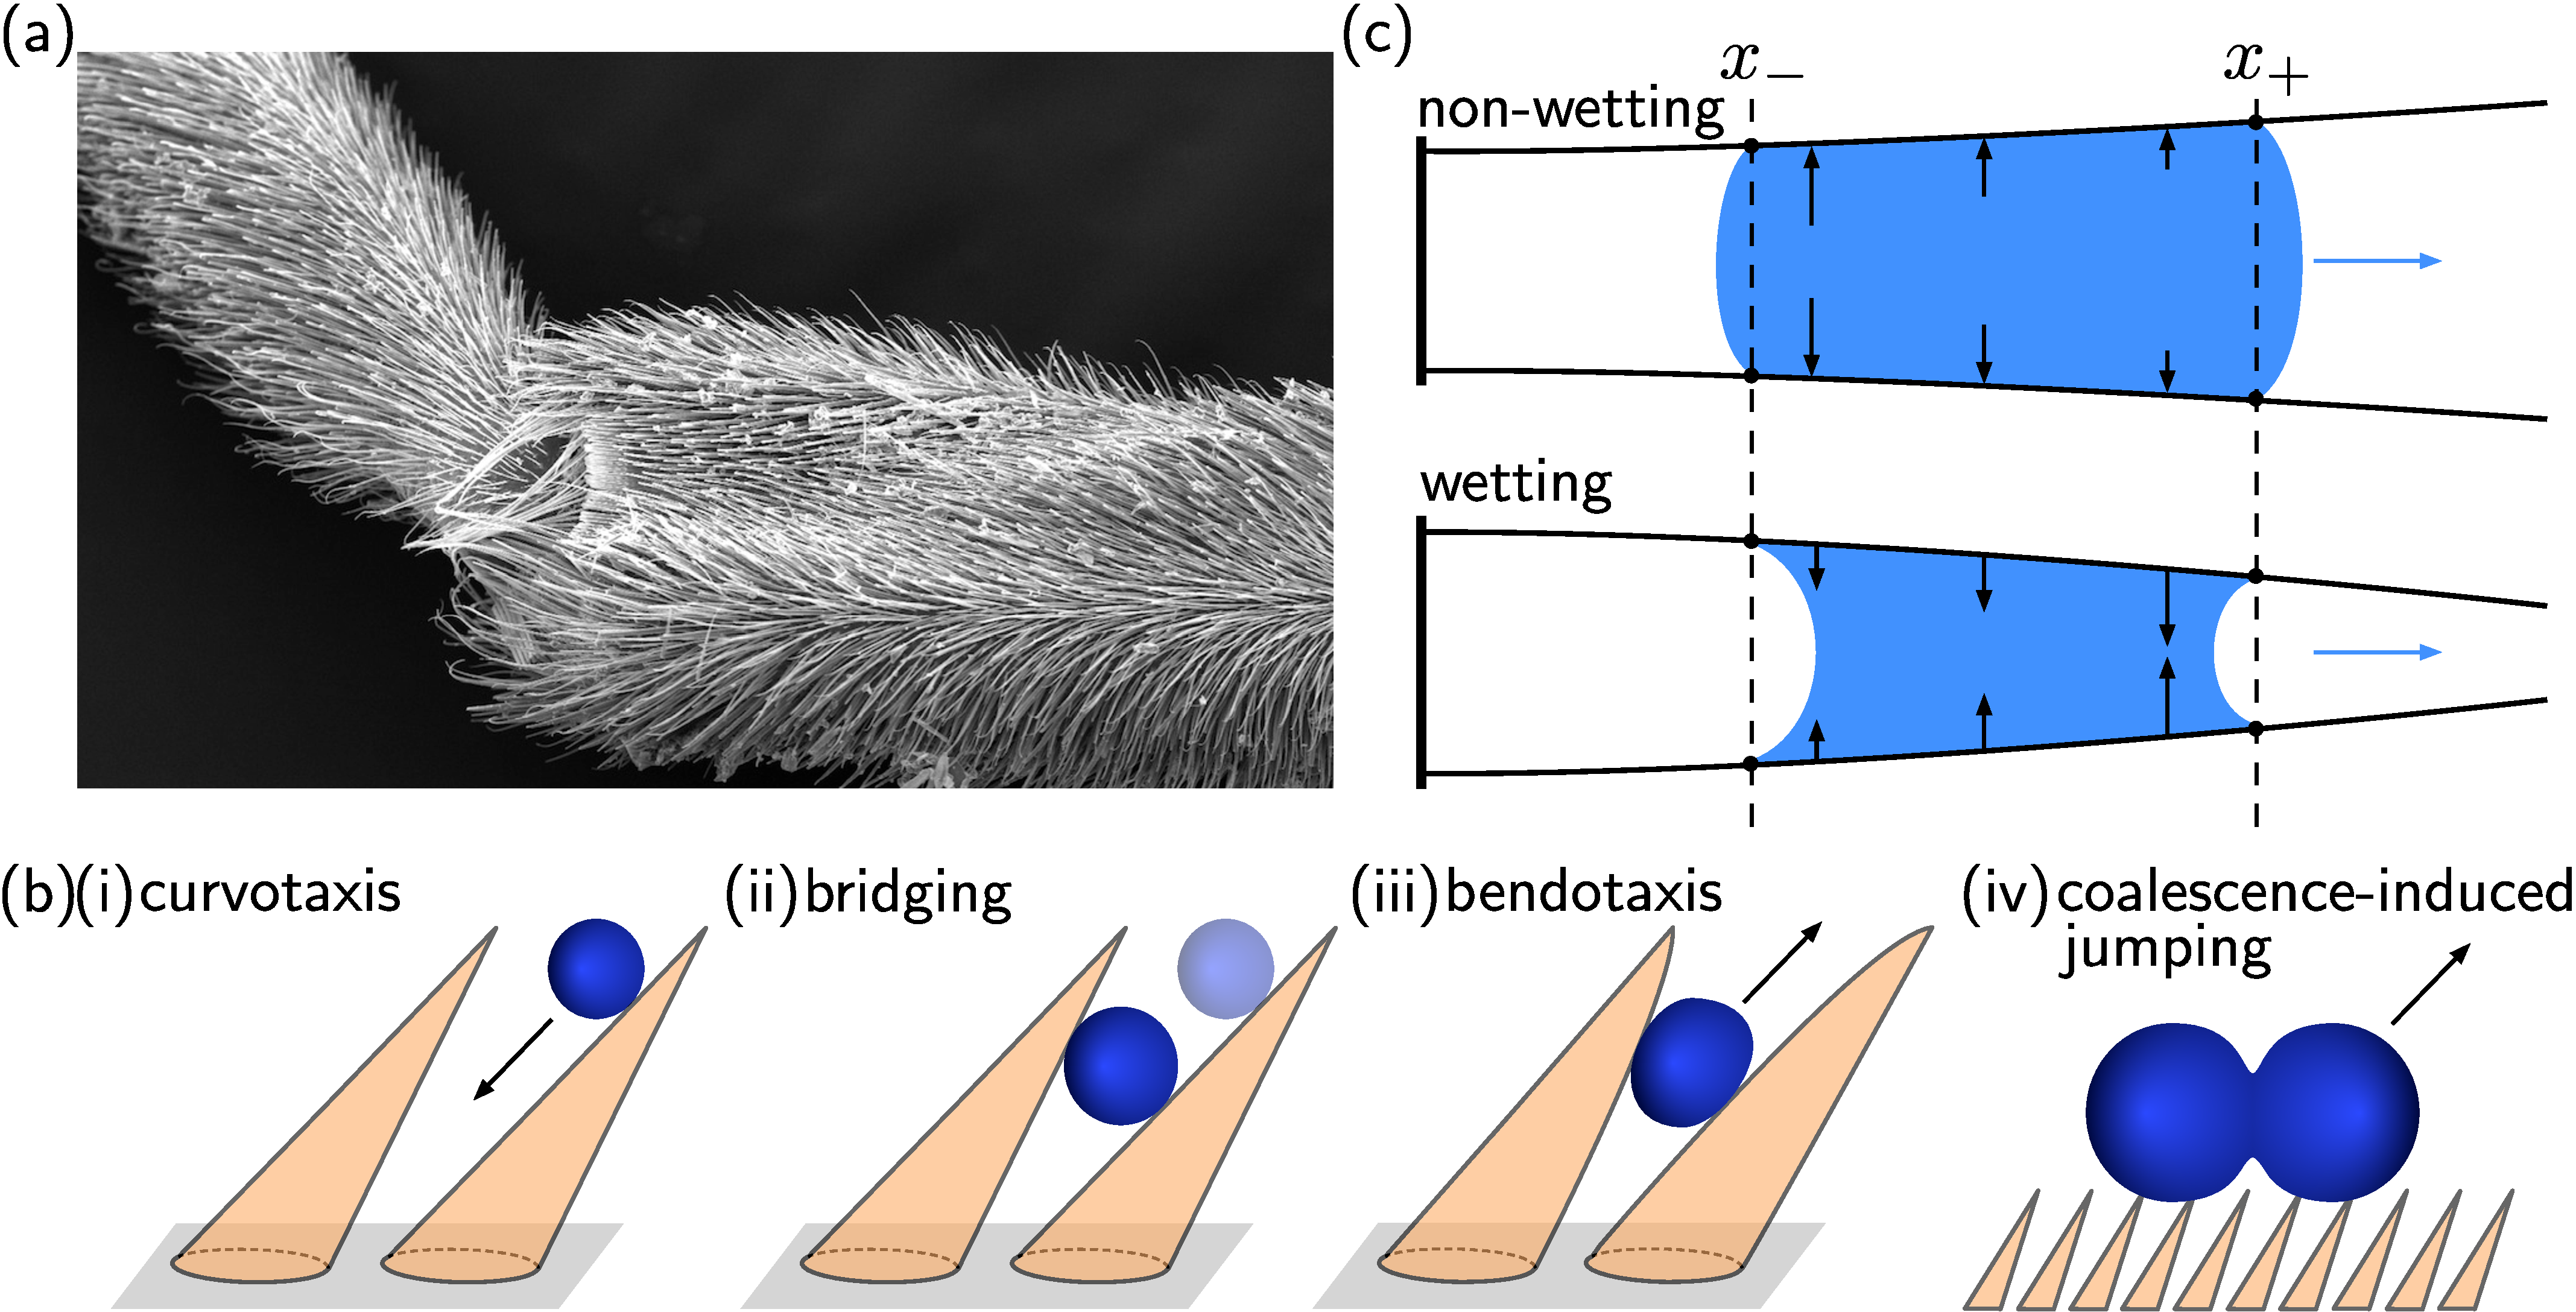
\includegraphics[width = \textwidth]{wang_schematic}
\caption{(a) Electron microscope image of a portion of the setae covering a leg of a \textit{Gerris Regimis} (or Water Strider). Collectively, the setae are responsible for the macroscopic superhydrophobicity of the leg. Image used with permission from Corinne Sommi/Swathmore College. (b) Schematic diagram of droplet removal from a channel between the setae on the leg of a water strider~\citep[after][]{Wang2015PNAS}. (i) The droplet moves along a conical seta to the narrower end of the channel via curvotaxis before (ii) contacting a neighbouring seta, all the while growing in size (via condensation). (iii) The droplet is expelled from the channel via bendotaxis (see main text), and it can subsequently be removed from the surface (iv) by coalescing with another droplet, for example. (c) Schematic diagrams explain the mechanism behind bendotaxis for non-wetting (top) and wetting (bottom) droplets. Black arrows indicate (schematically) the sign and magnitude of the Laplace pressure within the drop; blue arrows show the direction of decreasing pressure and hence droplet motion.}\label{fig:Ch1:StriderMechanism}
\end{figure}


Our inspiration for studying bendotaxis comes from recent observations of the legs of the \textit{Gerris Regimis} (commonly referred to as a Water Strider, or Pond Skater) by~\cite{Wang2015PNAS}. Water strider legs are covered in an array of conically shaped hairs (Figure~\ref{fig:Ch1:StriderMechanism}(a)), or setae. Collectively, the setae are responsible for the leg's superhydrophobicity by maintaining a Cassie-Baxter state~\citep{Gao2004Nature, Bush2006AnnRevFluidMech}. Superhydrophobicity is in turn important in reducing the energy required by the Water Strider to jump at the interface~\citep{Lee2009JFM}.

\cite{Wang2015PNAS} showed that the geometry and flexibility of the setae prevent the superhydrophobic leg from losing its water repellancy in the high humidity conditions in which the Water Strider dwells (where condensation of droplets would be an issue). As described by~\cite{Wang2015PNAS}, condensed droplets are removed from the setae in a three part process that is shown schematically in Figure~\ref{fig:Ch1:StriderMechanism}(b): firstly, a droplet of condensed water contacts a single seta and moves towards its base via curvotaxis. This phase ends with the droplet also contacting a neighbouring seta, forming a capillary bridge and effectively confining itself. The positive Laplace pressure of the droplet (water is non-wetting on the setae) then deforms this `channel' outwards, creating a geometric gradient that propels the non-wetting droplet towards regions of weaker confinement; this propulsion in response to droplet-induced channel deformations is caused by bending and hence we refer to it as bendotaxis.  Once the droplet has reached the tip, it can be removed (for example, by coalescence-induced jumping, as discussed in \S\ref{S:Ch1:superhydrophobic}).

%
%\blue{also a hat tip to Otten 2004 and Bernandino 2010 who argued about whether the flexiblity of the hairs on the Lady mantle aids with superhydrophobicity: could flexbility also help in another way?}


\subsection{Bendotaxis mechanism}
The geometry of a capillary bridge between conical setae is complicated. Moreover, the tapered channel formed by the conical fibres would expel the droplet, even in the absence of bending deformation. Therefore, to understand the mechanism of bendotaxis, and to isolate the role of bending alone, we consider the simplified scenario shown in Figure~\ref{fig:Ch1:StriderMechanism}(c): two, initially parallel, bendable walls are clamped at one end and free at the other. These two walls together form a two-dimensional channel.

If a wetting droplet is introduced between the walls, the interfacial curvature is negative at both ends of the droplet and the associated negative Laplace pressure deflects the walls inward (Figure~\ref{fig:Ch1:StriderMechanism}(c)).   The anisotropic boundary conditions (clamping at one end, free at the other) result in a channel that is effectively stiffer closer to the clamped end -- the same force applied closer to the clamped end results in a smaller deformation. As a result of this anisotropy, the channel deformation is larger at the meniscus closer to the free end (denoted $x_+$) than at the meniscus closer to the clamped end (denoted $x_-$). The pressure is therefore smaller (it is `more negative') at $x_+$ than at $x_-$, and the resulting pressure gradient drives the droplet towards the free end. Provided the contact angles remain the same and the walls do not touch, this motion will continue until the droplet reaches the free end.

If, however, a non-wetting droplet is introduced between the walls (as is the case in the setae of the water strider~\citep{Wang2015PNAS}), the Laplace pressure within the droplet is positive, pushing the walls away from one another (Figure~\ref{fig:Ch1:StriderMechanism}(c)). Again, however,  the resulting pressure gradient is negative, driving the droplet towards the free end. This argument suggest that  bendotaxis is wettability independent, the direction of motion is universal. (This thought experiment also clarifies the name bendotaxis: without channel flexibility, the pressure within the droplet would be constant and the droplet would be stationary. The droplet itself generates the tapering that leads to its motion.)

We can also view bendotaxis from an energetic perspective in this simple geometry. In the wetting case, the droplet would like to advance because the additional inwards deformation that results from this (the pressure applies at a distance further from the clamped end) will increase the length over which the droplet wets the channel (by conservation of droplet volume). Of course, this additional deformation incurs a bending energy penalty, but we shall see that, provided the channel walls do not touch, this penalty is not large enough to discourage the droplet from advancing. Similarly, in the non-wetting case, the outwards deformation that would result from the droplet's advance would lead to wetting over a shorter length, which is again energetically favourable.

It is the wettability-independence that makes it appealing to exploit bendotaxis in textured superhydrophobic surfaces: both wetting and non-wetting droplets would be spontaneously propelled towards the free end of the channel (i.e.~away from the surface, which would naturally correspond to the clamped end); this is in contrast to the rigid conically textured surfaces, in which only non-wetting droplets that bridge between cones are propelled away from the surface.

\subsection{Proof of concept}
\begin{figure}[t]
\centering
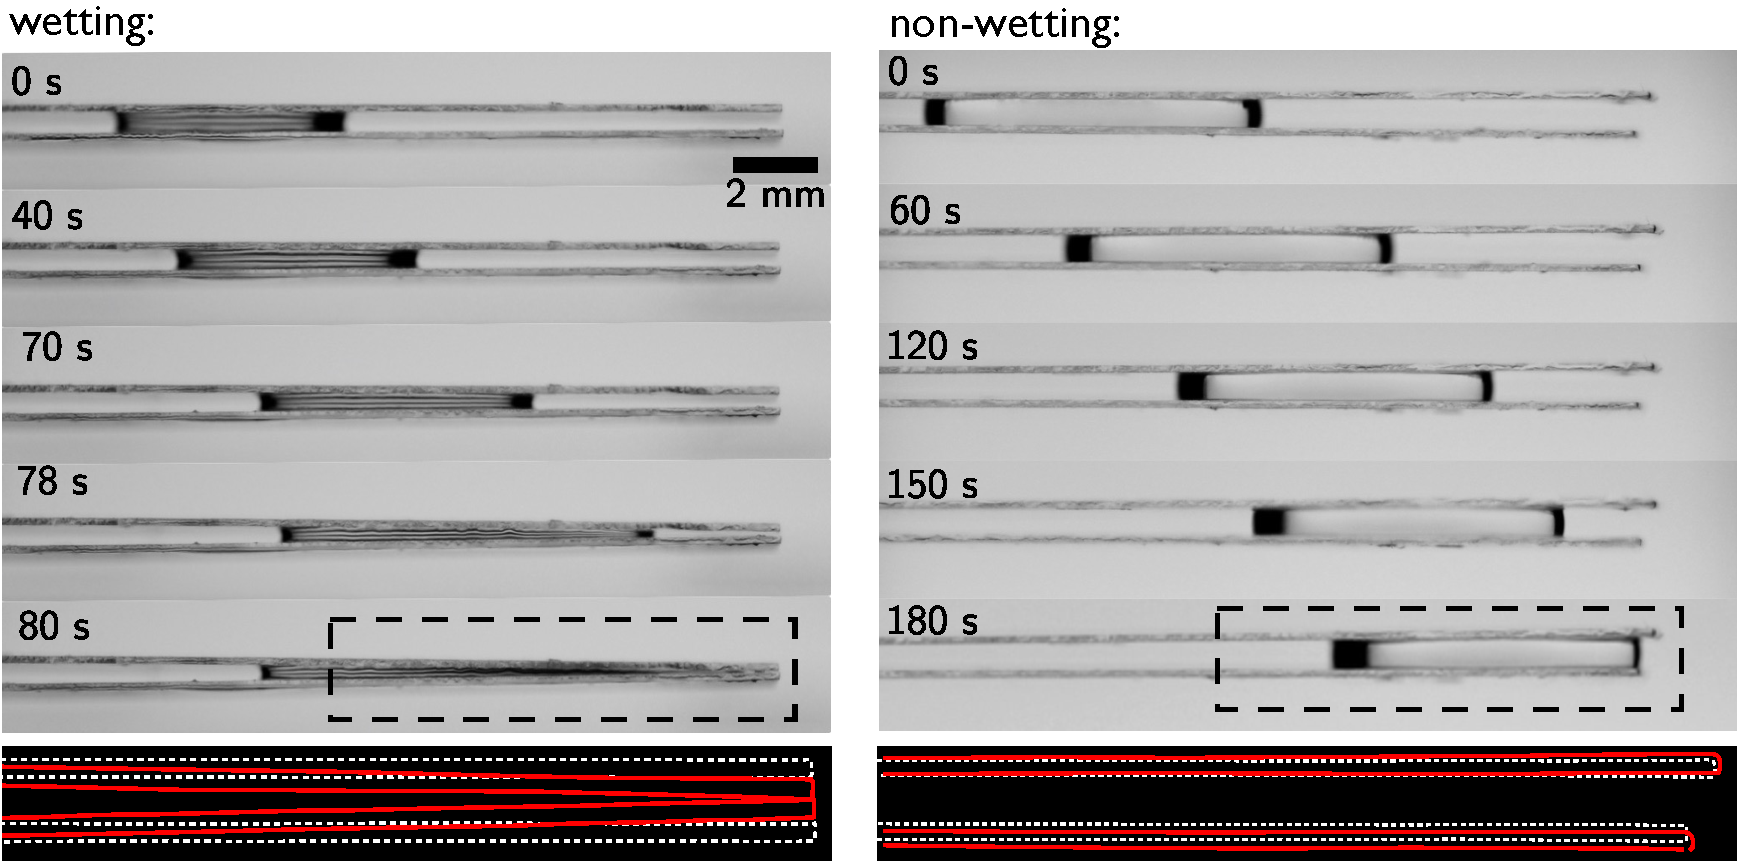
\includegraphics[width = \textwidth]{PoC_expts}
\caption{(top) Experimental demonstration of bendotaxis for a wetting silicone oil droplet (left) and a non-wetting water droplet (right), each between initially parallel, yet deformable, glass cover slips. While the deformation of the channel occurs in the opposite sense in each case (left: inwards, versus right: outwards), the direction of droplet motion is the same. (bottom) Comparison of final channel shape (red lines) with the initial channel shape (dotted white lines) for the section highlighted by the dashed box in the final experiment image.}\label{fig:Ch1:PoC}
\end{figure}


The bendotaxis mechanism described in  \S1.4.2 is reproducible in a simple laboratory experiment, with a channel fabricated using a rigid separator and glass cover slips. Figure~\ref{fig:Ch1:PoC} shows the time series of a wetting silicone oil droplet and of a non-wetting water droplet in such a channel. In both cases, the droplets move towards the free end of the channel. (More experimental details are given in Chapter 3.)

To observe the deflection of the cover slips, we compare their shapes in the final configuration with those prior to the introduction of the droplet (last panel in Figure~\ref{fig:Ch1:PoC}). In the wetting case, both cover slips are deflected inwards, while in the non-wetting case both are deflected outwards -- the deflections are in accord with the above physical description. The observed deflections also provide evidence that motion is not simply caused by the weight of the droplet, which would cause the lower cover slip to deflect downwards in both cases.

%describe what we do in the first half
In the first half of this thesis, we consider the quasi-two-dimensional configuration shown in Figure~\ref{fig:Ch1:PoC} and describe the dynamics of bendotaxis. With a view to the applicability of bendotaxis to anti-fogging surfaces, we focus on the time taken for droplets to be transported. We also consider situations in which the droplet transport is inhibited. Below we provide a more detailed synopsis of the three chapters that make up this first half.

In Chapter 2, we develop a two-dimensional mathematical model for bendotaxis. The physical processes represented by this model are motivated by those relevant in the proof of concept experiments in Figure~\ref{fig:Ch1:PoC}; in particular, we exploit the small aspect ratio of the channel and slenderness of its walls to combine lubrication theory and linear beam theory. By solving the model equations numerically, we verify that our model predicts wettability-independent droplet transport and gain insight into its dynamics; these numerical solutions are contrasted to analytic solutions available in the case of small channel deformations. Finally, we discuss the implications of our model for superhydrophobic surfaces that exploit bendotaxis.

In Chapter 3, we describe an experimental study of bendotaxis. The configuration is the similar to that for the experiments shown in Figure~\ref{fig:Ch1:PoC}, but we systematically vary the channel length, channel thickness, wall bending stiffness, wettability conditions, and liquid viscosity; these experiments provide a robust test of the mathematical model developed in Chapter 2 and offer further insight into the dynamics of bendotaxis.

In Chapter 4, we extend our mathematical model to include two phenomena encountered in Chapters 2 and 3 that can impede droplet transport: firstly, the scenario in which the channel walls touch before the droplet has reached the free end, trapping it indefinitely (so called `geometric trapping'), and, secondly, contact angle hysteresis, which, when sufficiently large, can completely arrest motion. For each of these, we describe the influence on the dynamics, and quantify when the droplet is prevented from reaching the free end. (Each of these effects would be detrimental to the performance of an anti-fogging textured surface exploiting bendotaxis).

\subsection{Bendotaxis in microchannels}

\begin{figure}
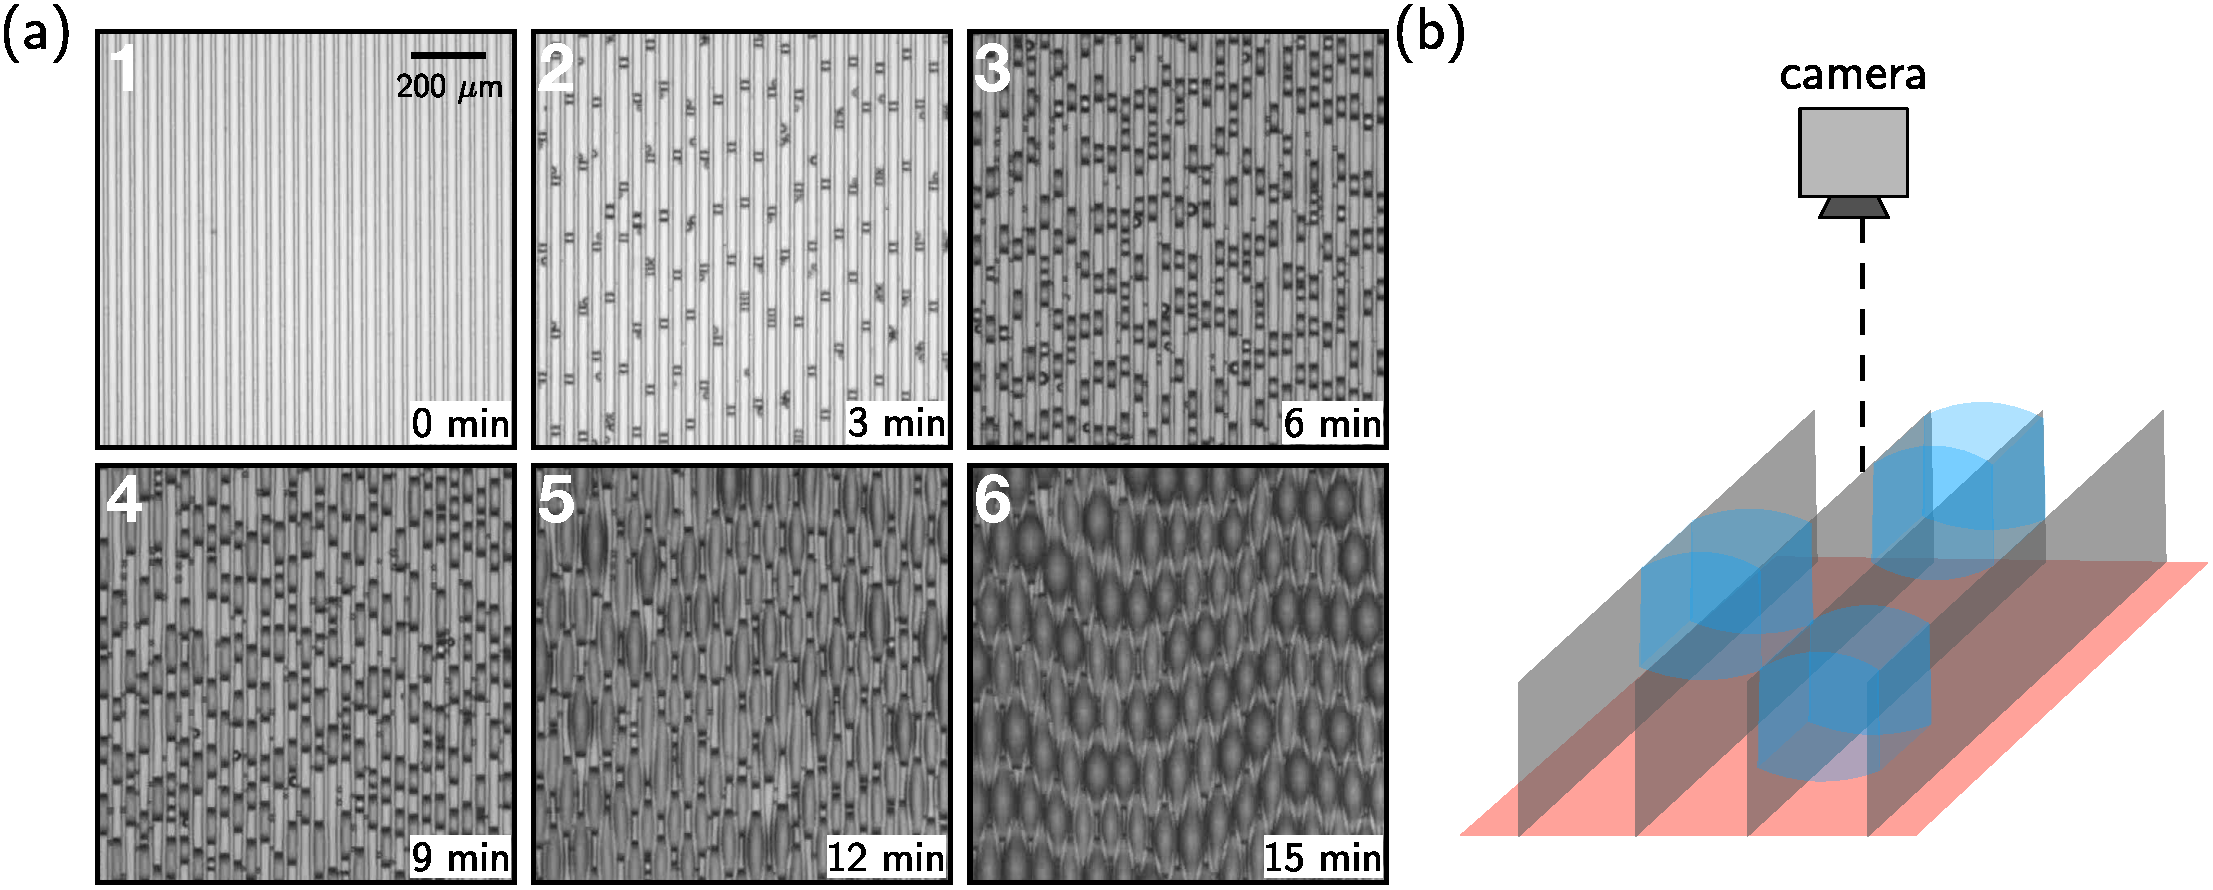
\includegraphics[width =0.95\textwidth]{BrinkmannExperiments}
\caption{Snapshots of experiments performed by~\cite{Seemann2011JPhysCondMat}. Droplets are condensed into an array of initially empty (1), deformable microchannels (the channel walls run vertically in the images, and the setup is shown schematically in (b)). Droplets continue to grow and move towards the open end (out of the page) of the channels (3, 4). Once droplets reach the end closest to the camera (5), their interface curvature relaxes and the light spot in their centre is no longer visible. The final configuration (6) has a lattice-like pattern charaterized by a pairwise mode in the direction perpendicular to the channel walls, as well as a periodic pattern in the parallel direction. We anticipate that this instability shares many features of bendotaxis.}\label{fig:Ch1:MBexpts}
\end{figure}

In the second half of this thesis, we consider how various channel geometries affect the bendotaxis mechanism. Motivation is provided the experiments of~\cite{Seemann2011JPhysCondMat} in which droplets are condensed into micro-channels. These experiments, shown in Figure~\ref{fig:Ch1:MBexpts}, clearly show an instability, and we shall explore the extent to which this instability may illustrate bendotaxis. In addition, these experiments may offer insight into how a superhydrophobic surface whose topographical features exploit bendotaxis to stay fog free might behave. (Superhydrophobic surfaces with flexible topographies have been realised~\citep[see][for example]{Blow2010Langmuir}, but typically do not have the correct geometry to exploit bendotaxis, with features too well separated from one another.)

As seen in the snapshots of these experiments (Figure~\ref{fig:Ch1:MBexpts}(a)), droplets nucleate at the base of a three dimensional array of channels and their upper surface moves towards the free end of the channels (the end closest to the camera, see Figure~\ref{fig:Ch1:MBexpts}(b)). This motion is reminiscent of bendotaxis; in particular, in both the wetting and non-wetting cases, this advancing interface is accompanied by a reduction in liquid pressure there (the channel deformation increases), encouraging flow towards it. While the interface is advancing, the volume of liquid in the channels is increasing as condensation continues. The motion of the (non-wetting) droplets can be inferred from the light patterns within them: when they are between the base and the free end, their interface curvature focusses incoming light and we see a bright spot in their centres (Figure~\ref{fig:Ch1:MBexpts}(a)2--5); once they touch the free end, the interfacial curvature of the droplets relaxes, resulting in a uniform light pattern on their surface (Figure~\ref{fig:Ch1:MBexpts}(a)6).

These experiments pose two questions: firstly, what controls the `weaving' instability seen in Figure~\ref{fig:Ch1:MBexpts}(a)? In Chapter 5, we study a previously-unreported instability mechanism, closely related to the Rayleigh--Plateau instability~\citep{Plateau1873, Rayleigh1879PRSL, Rayleigh1892PhilosMag}  whose mode selection may explain the length scale of this weaving instability.  We develop a mathematical model of a system that exhibits similar behaviour to gain insight into the dynamics of this instability, and describe the influence of the speed at which liquid is condensed into the channels on the mode selection problem.

The second question posed by the experiments of Figure~\ref{fig:Ch1:MBexpts} is: how would multiple droplets in neighbouring channels affect each other's bendotaxis? The deformation resulting from the Laplace pressure of condensed droplets changes not only the width of the channel that contains it, but also the width of the neighbouring channels. For a non-wetting liquid, the neighbouring channels are narrowed, tending to move droplets in those channels towards the base. In turn, this affects the thickness of the next-nearest neighbour to the original channel. By iterating this argument, we might expect a long range ordering in the direction perpendicular to the channel walls. Why then does this happen in a pairwise manner in the experiments of Figure~\ref{fig:Ch1:MBexpts}(a)? In Chapter 6 we describe the interaction between neighbouring channels, each of which would undergo bendotaxis in isolation and use this information to understand the clustering behaviour.

In Chapter 7, we summarize the main results of the thesis and discuss the possibilities for future work.
